\documentclass[11pt,a4paper]{article}
\usepackage[utf8]{inputenc}
\usepackage[T1]{fontenc}
\usepackage{amsmath}
\usepackage{amssymb}
\usepackage{amsfonts}
\usepackage{graphicx}
\usepackage[spanish]{babel}
\usepackage{booktabs, fourier, tabularx, wrapfig, multicol,multirow,caption, subcaption,tikz, fancyhdr, steinmetz, xcolor}
\usepackage[many]{tcolorbox}

\usepackage[left=2cm,right=2cm,top=2cm,bottom=2cm]{geometry}

\graphicspath{{./img/}}

%Acá voy a probar la rama
%%Acá va la segunda parte

%Configuración y comandos

%tcolorbox personalizado
\newtcolorbox{cajita}{colback=white!97!brown, colframe=brown!15!gray, breakable}

%Encabezado y pie de página
\fancyhead[R]{\textsc{Máquinas Eléctricas}}
\fancyhead[L]{
\includegraphics[width=.1\textwidth]{utncom}}
\fancyhead[C]{Hoja de fórmulas}
\fancyfoot[R]{ \vspace{.1cm} Página \thepage }
\fancyfoot[L]{\hrule \vspace{.1cm} Ingeniería Electromecánica}
\fancyfoot[C]{ \vspace{.1cm}}

\newtcolorbox{mybox}[1]{title = \textsc{Unidad #1},colbacktitle=red!85!black,enhanced,attach boxed title to top center={yshift=-2mm}, colbacktitle=white, coltitle=gray!50!black, boxed title style={colframe=blue!30},colback=white!97!brown, colframe=blue!30}

%Comando para fasores :)
\newcommand{\fasor}[1]{\uppercase{\textit{\textbf{#1}}}}
%Comando título de cada unidad
\newcommand{\unidad}[2]{\begin{center}
		\fontsize{10}{10}\selectfont\color{gray!50!black}\scshape Unidad #1 \\
		\fontsize{14}{14}\selectfont \scshape #2
\end{center} \vspace{-.6cm}}
%Comando pra subtitulos
\newcommand{\subtitulo}[1]{
    \textbf{#1} \\ \vspace{.1cm} {\color{gray} \hrule}
}

\begin{document}
    \pagestyle{fancy}
    \section*{Nomenclatura}
    \begin{tabular}{r l r l}
		$\fasor{Z}$ [$\Omega$]& Impedancia &
		$\fasor{i}$ [A] & Corriente \\
		$\fasor{v}$ [V] & Tensión&
		$j$ & Unidad imaginaria \\
		$t$ [s] & Tiempo &
		$P$ [W] & Potencia activa \\
		$Q$ [VAr] & Potencia reactiva &
		$\fasor{s}$ [VA] & Potencia aparente \\
        $m$ & Relación de transformación&
        $\fasor{I}_{exc}$ o $\fasor{I}_0$ [A] & Corriente de excitación\\
        $\fasor{I}_{Fe}$ [A] & Corriente debido a pérdidas en el Fe&
        $\fasor{I}_{\mu}$ [A] & Corriente magnetizante\\
	\end{tabular}
    \unidad{1}{Acá quiero poner lo de las bobinas y eso... VER}
    \unidad{2}{Transformadores}

    \begin{cajita}
        \centering
        \begin{center}
            \subtitulo{Transformador Ideal \textnormal{en vacío}}
        \end{center}
        \vspace{-.3cm} \textsc{sin pérdidas} \vspace{.1cm}

        \begin{tabular}{r l}
            Autoinducción & $L = \dfrac{\mu N^2 S}{l}$ \\
        \end{tabular} \vspace{.4cm}

        \textsc{con pérdidas} \vspace{.1cm}

        \begin{tabular}{r l}
            \multicolumn{2}{c}{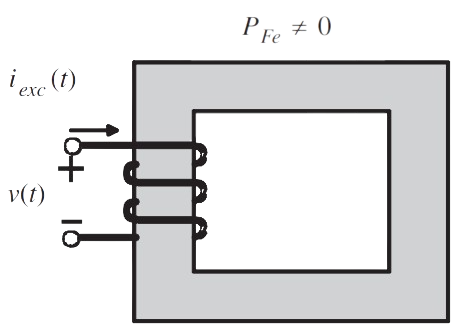
\includegraphics[width = 4cm]{vacio-cp-trafo}  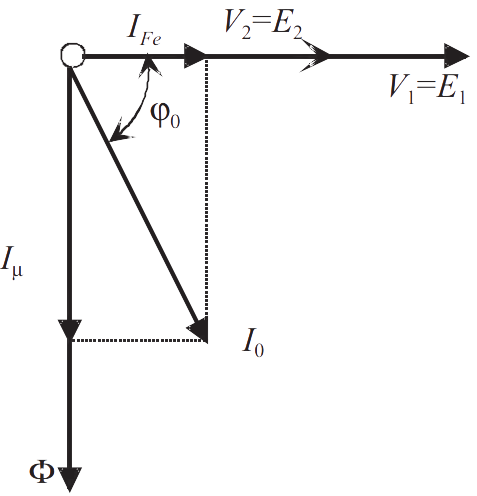
\includegraphics[width = 2.5cm]{vacio-fasores}} \\
            Fem & $\mathcal{F} = N_1  \fasor{i}_1  = N_1  \fasor{i}_0$\\
            Relación de transfor. & $m = \dfrac{E_1}{E_2} = \dfrac{V_1}{V_2}$ \\
            \multicolumn{2}{c}{$ \fasor{i}_0 = \fasor{i}_\mu + \fasor{i}_{Fe} $} \\
        \end{tabular}
        
        \begin{center}
            \subtitulo{Transformador Ideal \textnormal{en carga}}
        \end{center}
        \begin{tabular}{r l}
            \multicolumn{2}{c}{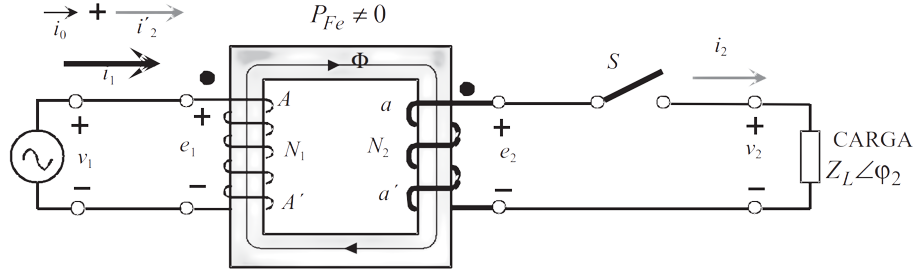
\includegraphics[width = 6cm]{carga-trafo}} \\
            Fem & $\mathcal{F} = N_1  \fasor{i}_1 - N_2 \fasor{i}_2$\\
            & $\fasor{i}_0 = \fasor{i}_1 - \dfrac{N_2}{N_1} \fasor{i}_2$\\
            Corriente reducida & $\fasor{i'}_2 = \dfrac{\fasor{i}_2}{m}$ \\
        \end{tabular}

    \end{cajita}

\end{document}